\documentclass[a4paper]{scrreprt}
\usepackage{fancyhdr}
\pagestyle{fancy}
\usepackage[english]{babel}
\usepackage[utf8]{inputenc}
\usepackage{graphicx}
\usepackage{url}
\usepackage{textcomp}
\usepackage{amsmath}
\usepackage{lastpage}
\usepackage{pgf}
\usepackage{wrapfig}
\usepackage{fancyvrb}
\usepackage{appendix}
\usepackage{pdfpages}
\usepackage{xcolor}
\usepackage{hyperref}

\hypersetup{
    colorlinks=true,
    linkcolor=blue,
    filecolor=black,      
    urlcolor=blue,
    citecolor=black,
}

% Create header and footer
\headheight 27pt
\pagestyle{fancyplain}
\lhead{\footnotesize{Datalagring, IV1351}}
\chead{\footnotesize{Seminar 1}}
\rhead{}
\lfoot{}
\cfoot{\thepage\ (\pageref{LastPage})}
\rfoot{}

% Create title page
\title{Seminar 1}
\subtitle{Datalagring, IV1351}
\author{Adrian Jonsson Sjödin \\ adriansj@kth.se}
\date{\today} 


\begin{document}

\maketitle

\tableofcontents %Generates the TOC

\chapter{Introduction}
The purpose of this seminar is to practice modeling information based on an organizational description that will later be turned into a functioning database. The first
step in this is to produce a conceptual model. The creation and reasoning behind this conceptual model is what will be covered in this report.

\chapter{Method}



\begin{figure}[h]
    \begin{center}
        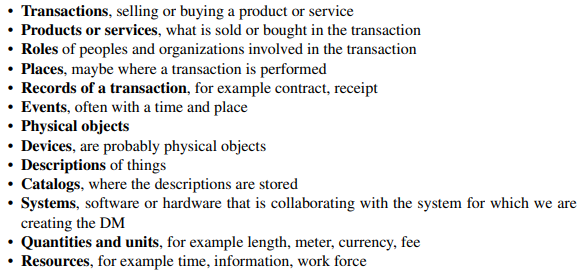
\includegraphics[scale = 1.0 ]{../img/CategoryList.PNG}
        \caption{Category list. \\ \textit{L Lindbäck, A First Course in Object Oriented Development, A Hands-On Approach, 2022}}
        \label{fig:categoryList}
    \end{center}
\end{figure}



\chapter{Result}
\label{sec:result}




\chapter{Discussion}


\end{document}
